\documentclass[twoside,11pt]{article}

% ? Specify used packages
\usepackage{graphicx}        %  Use this one for final production.
% \usepackage[draft]{graphicx} %  Use this one for drafting.
% ? End of specify used packages

\pagestyle{myheadings}

% -----------------------------------------------------------------------------
% ? Document identification
\newcommand{\stardoccategory}  {Starlink User Note}
\newcommand{\stardocinitials}  {SUN}
\newcommand{\stardocsource}    {sun\stardocnumber}
\newcommand{\stardocnumber}    {189.3}
\newcommand{\stardocauthors}   {Martin Clayton}
\newcommand{\stardocdate}      {25 June 1996}
\newcommand{\stardoctitle}     {ISPELL \sunspec{--}{-} Spelling Checker}
\newcommand{\stardocversion}   {[software-version]}
\newcommand{\stardocmanual}    {[manual-type]}
\newcommand{\stardocabstract}  {[Text of abstract]}
% ? End of document identification

% -----------------------------------------------------------------------------

\newcommand{\stardocname}{\stardocinitials /\stardocnumber}
\markright{\stardocname}
\setlength{\textwidth}{160mm}
\setlength{\textheight}{230mm}
\setlength{\topmargin}{-2mm}
\setlength{\oddsidemargin}{0mm}
\setlength{\evensidemargin}{0mm}
\setlength{\parindent}{0mm}
\setlength{\parskip}{\medskipamount}
\setlength{\unitlength}{1mm}

% -----------------------------------------------------------------------------
%  Hypertext definitions.
%  ======================
%  These are used by the LaTeX2HTML translator in conjunction with star2html.

%  Comment.sty: version 2.0, 19 June 1992
%  Selectively in/exclude pieces of text.
%
%  Author
%    Victor Eijkhout                                      <eijkhout@cs.utk.edu>
%    Department of Computer Science
%    University Tennessee at Knoxville
%    104 Ayres Hall
%    Knoxville, TN 37996
%    USA

%  Do not remove the %begin{latexonly} and %end{latexonly} lines (used by
%  LaTeX2HTML to signify text it shouldn't process).
%begin{latexonly}
\makeatletter
\def\makeinnocent#1{\catcode`#1=12 }
\def\csarg#1#2{\expandafter#1\csname#2\endcsname}

\def\ThrowAwayComment#1{\begingroup
    \def\CurrentComment{#1}%
    \let\do\makeinnocent \dospecials
    \makeinnocent\^^L% and whatever other special cases
    \endlinechar`\^^M \catcode`\^^M=12 \xComment}
{\catcode`\^^M=12 \endlinechar=-1 %
 \gdef\xComment#1^^M{\def\test{#1}
      \csarg\ifx{PlainEnd\CurrentComment Test}\test
          \let\html@next\endgroup
      \else \csarg\ifx{LaLaEnd\CurrentComment Test}\test
            \edef\html@next{\endgroup\noexpand\end{\CurrentComment}}
      \else \let\html@next\xComment
      \fi \fi \html@next}
}
\makeatother

\def\includecomment
 #1{\expandafter\def\csname#1\endcsname{}%
    \expandafter\def\csname end#1\endcsname{}}
\def\excludecomment
 #1{\expandafter\def\csname#1\endcsname{\ThrowAwayComment{#1}}%
    {\escapechar=-1\relax
     \csarg\xdef{PlainEnd#1Test}{\string\\end#1}%
     \csarg\xdef{LaLaEnd#1Test}{\string\\end\string\{#1\string\}}%
    }}

%  Define environments that ignore their contents.
\excludecomment{comment}
\excludecomment{rawhtml}
\excludecomment{htmlonly}

%  Hypertext commands etc. This is a condensed version of the html.sty
%  file supplied with LaTeX2HTML by: Nikos Drakos <nikos@cbl.leeds.ac.uk> &
%  Jelle van Zeijl <jvzeijl@isou17.estec.esa.nl>. The LaTeX2HTML documentation
%  should be consulted about all commands (and the environments defined above)
%  except \xref and \xlabel which are Starlink specific.

\newcommand{\htmladdnormallinkfoot}[2]{#1\footnote{#2}}
\newcommand{\htmladdnormallink}[2]{#1}
\newcommand{\htmladdimg}[1]{}
\newenvironment{latexonly}{}{}
\newcommand{\hyperref}[4]{#2\ref{#4}#3}
\newcommand{\htmlref}[2]{#1}
\newcommand{\htmlimage}[1]{}
\newcommand{\htmladdtonavigation}[1]{}

% Define commands for HTML-only or LaTeX-only text.
\newcommand{\html}[1]{}
\newcommand{\latex}[1]{#1}

% Use latex2html 98.2.
\newcommand{\latexhtml}[2]{#1}

%  Starlink cross-references and labels.
\newcommand{\xref}[3]{#1}
\newcommand{\xlabel}[1]{}

%  LaTeX2HTML symbol.
\newcommand{\latextohtml}{{\bf LaTeX}{2}{\tt{HTML}}}

%  Define command to re-centre underscore for Latex and leave as normal
%  for HTML (severe problems with \_ in tabbing environments and \_\_
%  generally otherwise).
\newcommand{\setunderscore}{\renewcommand{\_}{{\tt\symbol{95}}}}
\latex{\setunderscore}

% -----------------------------------------------------------------------------
%  Debugging.
%  =========
%  Remove % from the following to debug links in the HTML version using Latex.

% \newcommand{\hotlink}[2]{\fbox{\begin{tabular}[t]{@{}c@{}}#1\\\hline{\footnotesize #2}\end{tabular}}}
% \renewcommand{\htmladdnormallinkfoot}[2]{\hotlink{#1}{#2}}
% \renewcommand{\htmladdnormallink}[2]{\hotlink{#1}{#2}}
% \renewcommand{\hyperref}[4]{\hotlink{#1}{\S\ref{#4}}}
% \renewcommand{\htmlref}[2]{\hotlink{#1}{\S\ref{#2}}}
% \renewcommand{\xref}[3]{\hotlink{#1}{#2 -- #3}}
%end{latexonly}
% -----------------------------------------------------------------------------
% ? Document-specific \newcommand or \newenvironment commands.
\newcommand{\sunspec}[2]{#1}
\begin{htmlonly}
\newcommand{\sunspec}[2]{#2}
\end{htmlonly}

% ? End of document-specific commands
% -----------------------------------------------------------------------------
%  Title Page.
%  ===========
\renewcommand{\thepage}{\roman{page}}
\begin{document}
\thispagestyle{empty}

%  Latex document header.
%  ======================
\begin{latexonly}
   CCLRC / {\sc Rutherford Appleton Laboratory} \hfill {\bf \stardocname}\\
   {\large Particle Physics \& Astronomy Research Council}\\
   {\large Starlink Project\\}
   {\large \stardoccategory\ \stardocnumber}
   \begin{flushright}
   \stardocauthors\\
   \stardocdate
   \end{flushright}
   \vspace{-4mm}
   \rule{\textwidth}{0.5mm}
   \vspace{5mm}
   \begin{center}
   {\Huge\bf  \stardoctitle \\ [2.5ex]}
%   {\LARGE\bf \stardocversion \\ [4ex]}
%   {\Huge\bf  \stardocmanual}
   \end{center}
   \vspace{5mm}

% ? Add picture here if required.
   \begin{center}
   \leavevmode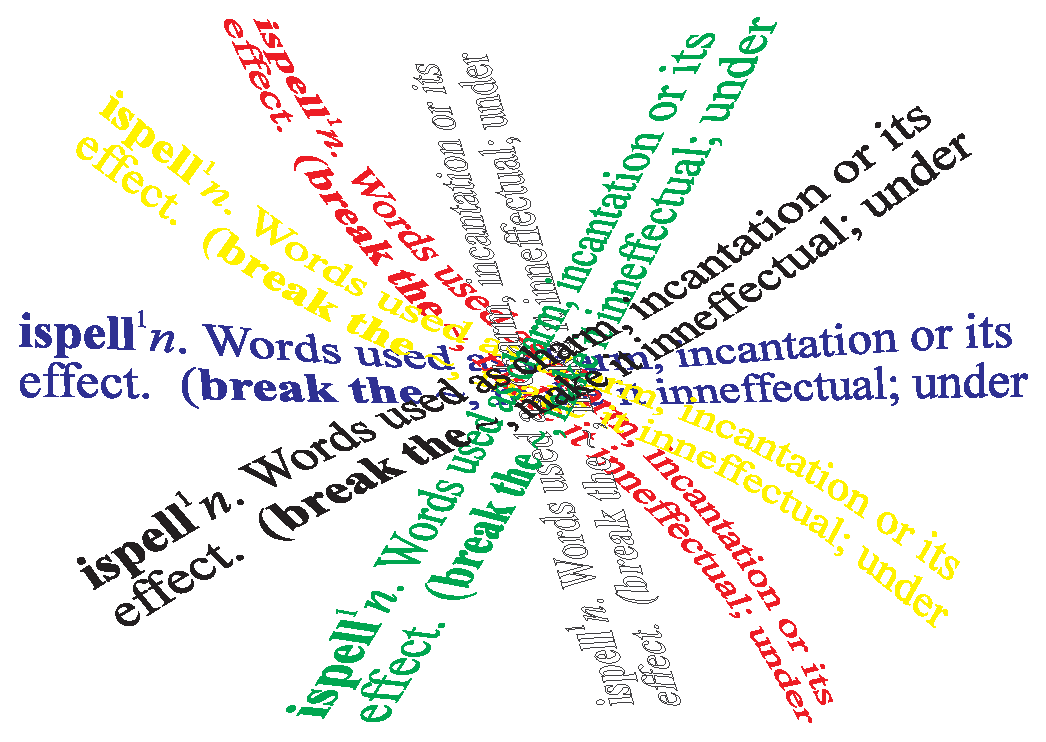
\includegraphics[height=100mm]{sun189_cover}
   \end{center}
% ? End of picture

% ? Heading for abstract if used.
%   \vspace{10mm}
%   \begin{center}
%      {\Large\bf Abstract}
%   \end{center}
% ? End of heading for abstract.
\end{latexonly}

%  HTML documentation header.
%  ==========================
\begin{htmlonly}
   \xlabel{}
   \begin{rawhtml} <H1> \end{rawhtml}
      \stardoctitle
   \begin{rawhtml} </H1> \end{rawhtml}

% ? Add picture here if required.
   \begin{figure}[h]
   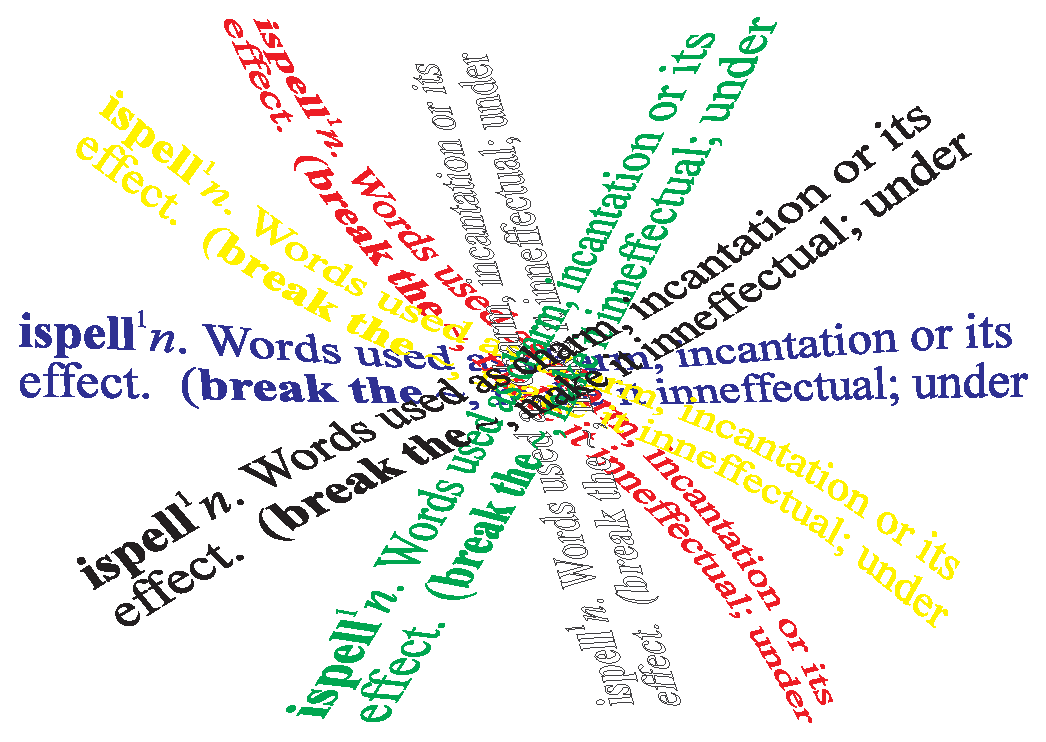
\includegraphics[height=100mm]{sun189_cover}
   \end{figure}
% ? End of picture

   \begin{rawhtml} <P> <I> \end{rawhtml}
   \stardoccategory\ \stardocnumber \\
   \stardocauthors \\
   \stardocdate
   \begin{rawhtml} </I> </P> <H3> \end{rawhtml}
      \htmladdnormallink{CCLRC}{http://www.cclrc.ac.uk} /
      \htmladdnormallink{Rutherford Appleton Laboratory}
                        {http://www.cclrc.ac.uk/ral} \\
      \htmladdnormallink{Particle Physics \& Astronomy Research Council}
                        {http://www.pparc.ac.uk} \\
   \begin{rawhtml} </H3> <H2> \end{rawhtml}
      \htmladdnormallink{Starlink Project}{http://www.starlink.ac.uk/}
   \begin{rawhtml} </H2> \end{rawhtml}
   \htmladdnormallink{\htmladdimg{source.gif} Retrieve hardcopy}
      {http://www.starlink.ac.uk/cgi-bin/hcserver?\stardocsource}\\

%  HTML document table of contents.
%  ================================
%  Add table of contents header and a navigation button to return to this
%  point in the document (this should always go before the abstract \section).
  \label{stardoccontents}
  \begin{rawhtml}
    <HR>
    <H2>Contents</H2>
  \end{rawhtml}
  \htmladdtonavigation{\htmlref{\htmladdimg{contents_motif.gif}}
        {stardoccontents}}

% ? New section for abstract if used.
%  \section{\xlabel{abstract}Abstract}
% ? End of new section for abstract
\end{htmlonly}

% -----------------------------------------------------------------------------
% ? Document Abstract. (if used)
%  ==================
%\stardocabstract
% ? End of document abstract
% -----------------------------------------------------------------------------
% ? Latex document Table of Contents (if used).
%  ===========================================
\newpage
\begin{latexonly}
   \setlength{\parskip}{0mm}
   \tableofcontents
   \setlength{\parskip}{\medskipamount}
   \markright{\stardocname}
\end{latexonly}
% ? End of Latex document table of contents
% -----------------------------------------------------------------------------
\newpage
\renewcommand{\thepage}{\arabic{page}}
\setcounter{page}{1}

\section{ISPELL in brief}

For a simple operation like checking the spelling in a text document, this User
Note may seem a bit long \sunspec{--}{-} however, this Section covers all the
basics.
Anyone familiar with the old VMS SPELL program will find ISPELL similar.

ISPELL is a screen-oriented spelling checker that shows errors in the context
of the original file, and suggests possible corrections when it can figure
them out.  The most common usage is

\begin{verbatim}
   % ispell filename
\end{verbatim}

In this case, ISPELL will display each word which does not appear in the
dictionary at the top of the screen and allow you to change it.
If there are `near misses' in the dictionary (words which differ by only a
single letter, a missing or extra letter, a pair of transposed letters, or a
missing space or hyphen), then they are also displayed on following lines.
As well as near misses, ISPELL may display other guesses at ways to make the
word from a known root, with each guess preceded by question marks.
The line containing the word and the previous line
are printed on the screen below the word itself. If your terminal can
display in reverse video, the word itself is highlighted.  You have the
option of replacing the word completely, or choosing one of the suggested
words.  A summary of the available user commands is displayed in a menu at the
bottom of the screen.

ISPELL will ignore \TeX\ and \LaTeX\ commands in files whose names end in
\verb+.tex+\@.  Non-simple user-defined environments may confuse ISPELL
causing spelling errors to be missed.
In this case the \verb+-n+ command-line option for ISPELL should be used.

If ISPELL does not detect any errors in the text file it will exit without
entering its interactive mode.


\section{About this User Note}

Most of the information in this document can be accessed on the ISPELL man page
by typing

\begin{verbatim}
   % man ispell
\end{verbatim}

There follows a complete list of the interactive commands available when
checking a document with ISPELL, and command-line options. A brief description
of the origin of the dictionary used in the Starlink release is also given.


\section{Interactive commands}

ISPELL accepts user inputs which are single-letter commands.  The
case of the commands is ignored.

Commands are as follows:

\begin{latexonly}
\begin{tabular}{ll}
Command & Description \\ \hline
{\tt ?    } & Display the help screen.\\
{\tt 0-n  } & Replace with one of the suggested words.\\
{\tt A    } & Accept the word for the rest of this ISPELL session.\\
{\tt I    } & Accept the word, capitalized as it is in the file, and update\\
            & the private dictionary.\\
{\tt L    } & Look up words in system dictionary.\\
{\tt Q    } & Exit immediately and leave the file unchanged.\\
{\tt R    } & Replace the misspelled word completely.\\
space       & Accept the word this time only.\\
{\tt U    } & Accept the word, and add an uncapitalised (actually, all
              lower-case)\\
            & version to the private dictionary.\\
{\tt X    } & Write the rest of this file, ignoring misspellings, and start the
              next file.\\
{\tt !    } & Shell escape.\\
ctrl-L      & Redraw screen.\\
ctrl-Z      & Suspend ispell.\\
\end{tabular}
\end{latexonly}
\begin{htmlonly}
\begin{rawhtml}
<PRE>
<B>Command   Description</B>
?         Display the help screen.
0-n       Replace with one of the suggested words.
A         Accept the word for the rest of this ISPELL session.
I         Accept the word, capitalized as it is in the file, and
          update the private dictionary.
L         Look up words in system dictionary.
Q         Exit immediately and leave the file unchanged.
R         Replace the misspelled word completely.
space     Accept the word this time only.
U         Accept the word, and add an uncapitalised (actually, all
          lower-case) version to the private dictionary.
X         Write the rest of this file, ignoring misspellings, and
          start the next file.
!         Shell escape.
ctrl-L    Redraw screen.
ctrl-Z    Suspend ispell.
</PRE>
\end{rawhtml}
\end{htmlonly}

\section{Command line arguments}

In brief, the available command-line arguments are:

\begin{latexonly}
\begin{tabular}{ll}
Argument & Description \\ \hline
{\tt -M       } & Display a one-line mini-menu in interactive mode.\\
{\tt -N       } & Do not display a one-line mini-menu in interactive mode.\\
{\tt -Ln      } & Display \verb+n+ lines of context in interactive mode.\\

{\tt -b       } & Create a backup file by appending \verb+.bak+ to the name of
                  the input file.\\
{\tt -x       } & Don't create a backup file.\\

{\tt -t       } & The input file is in \TeX\ or \LaTeX\ format.\\
{\tt -n       } & The input file is in nroff/troff format.\\

{\tt -B       } & Report run-together words with missing blanks as spelling
                  errors.\\
{\tt -C       } & Consider run-together words as legal compounds.\\

{\tt -P       } & Don't generate extra root/affix combinations.\\
{\tt -m       } & Make possible root/affix combinations that aren't in the
                  dictionary.\\

{\tt -s       } & Sort the list of guesses by probable correctness.\\
{\tt -d file  } & Specify an alternate dictionary \verb+file+\@.\\
{\tt -p file  } & Specify an alternate personal dictionary \verb+file+\@.\\
{\tt -w chars } & Specify additional characters \verb+chars+ that can be part
                  of a word.\\
{\tt -W n     } & Specify length \verb+n+ of words that are always legal.\\
{\tt -T type  } & Assume a given formatter type for all files.\\

{\tt -V       } & Display non-printing characters in \verb+cat -v+ style.\\
{\tt -l       } & Produce a list of misspelled words from the standard input.\\

{\tt -a       } & Run ISPELL in a pipe.\\
{\tt -A       } & As \verb+-a+ with nested file capability.\\
{\tt -f file  } & Write output to \verb+file+ (valid with \verb+-A+ and
                  \verb+-a+ only).\\

{\tt -v       } & Display version ID and licence then exit.\\
{\tt -vv      } & Display version ID, licence and compilation options then
                  exit.\\
\end{tabular}
\end{latexonly}

\begin{htmlonly}
\begin{rawhtml}
<PRE>
<B>Argument  Description</B>
-M        Display a one-line mini-menu in interactive mode.
-N        Do not display a one-line mini-menu in interactive mode.
-Ln       Display <B>n</B> lines of context in interactive mode.
-b        Create a backup file by appending <B>.bak</B> to the
          name of the input file.
-x        Don't create a backup file.
-t        The input file is in TeX or LaTeX format.
-n        The input file is in nroff/troff format.
-B        Report run-together words with missing blanks as
          spelling errors.
-C        Consider run-together words as legal compounds.
-P        Don't generate extra root/affix combinations.
-m        Make possible root/affix combinations that aren't in
          the dictionary.
-s        Sort the list of guesses by probable correctness.
-d file   Specify an alternate dictionary <B>file</B>.
-p file   Specify an alternate personal dictionary <B>file</B>.
-w chars  Specify additional characters <B>chars</B> that can be part of
          a word.
-W n      Specify length <B>n</B> of words that are always legal.
-T type   Assume a given formatter <B>type</B> for all files.
-V        Display non-printing characters in `cat -v' style.
-l        Produce a list of misspelled words from the standard input.
-a        Run ISPELL in a pipe.
-A        As -a with nested file capability.
-f file   Write output to <B>file</B> (valid with <B>-A</B> and <B>-a</B> only).
-v        Display version ID and licence then exit.
-vv       Display version ID, licence and compilation options then exit.
</PRE>
\end{rawhtml}
\end{htmlonly}

And in a little more detail:

\begin{itemize}
\item {\Large\tt -M} \\
If the \verb+-M+ switch is specified, a one-line mini-menu at the bottom of the
screen will summarize these options. By default the menu {\bf is} displayed.

\item {\Large\tt -N} \\
The \verb+-N+ switch may be used to suppress the one-line mini-menu.

\item {\Large\tt -Ln} \\
If the \verb+-L+ flag is given, the specified number,\verb+n+, is used as the
number of lines of context to be shown on the screen.  (The default is to
calculate the amount of context as a certain percentage of the screen
size).  The amount of context is subject to a system-imposed limit, typically
it depends how many lines your terminal will display.

\item {\Large\tt -b} \\
The \verb+-b+ option forces ispell to leave a backup \verb+.bak+ file for each
input file.
The \verb+.bak+ file contains the pre-corrected text.
A backup file {\bf is} left by default.

\item {\Large\tt -x} \\
The \verb+-x+ option suppresses the retention of the \verb+.bak+ files.
If there are file opening/writing errors, the \verb+.bak+ file may be left for
recovery purposes even with the \verb+-x+ option.

\item {\Large\tt -n} and {\Large\tt -t}\\
The \verb+-n+ and \verb+-t+ options select whether ISPELL runs in nroff/troff
(\verb+-n+) or \TeX /\LaTeX\ (\verb+-t+) input mode.
\TeX /\LaTeX\ mode is automatically selected if an input file has the extension
\verb+.tex+, unless overridden by the -n switch.
Files with extensions other than \verb+.tex+ will be assumed to {\bf not} be in
\TeX\ or \LaTeX\ format.
In \TeX /\LaTeX\ mode, whenever a backslash (``\verb+\+'') is found, ISPELL
will skip to the next whitespace or \TeX /\LaTeX\ delimiter.
Certain commands contain arguments which should not be checked, such as labels
and reference keys as are found in the \verb+\cite+ command, since they contain
arbitrary, non-word arguments.
Spell checking is also suppressed when in math mode.
Thus, for example, given

\begin{verbatim}
   \chapter {This is a Ckapter} \cite{SCH86}
\end{verbatim}

ISPELL will find \verb+Ckapter+ but not \verb+SCH+\@.
The \verb+-t+ option does not recognize the \TeX\ comment character \verb+%+,
so comments are also spell-checked.
It also assumes correct \LaTeX\ syntax.
Arguments to infrequently used commands and some optional arguments are
sometimes checked unnecessarily.

References for the \verb+tib+ bibliography system, that is, text between a
``[.'' or ``$<$.'' and ``.]'' or ``.$>$'' will always be ignored in \TeX /\LaTeX\
mode.

\item {\Large\tt -B} and {\Large\tt -C} \\
The \verb+-B+ and \verb+-C+ options control how ISPELL handles run-together
words, such as ``notthe'' for ``not the''\@.
If \verb+-B+ is specified, such words will be considered as errors, and
ISPELL will list variations with an inserted blank or hyphen as possible
replacements.
If \verb+-C+ is specified, run-together words will be considered to be legal
compounds, so long as both components are in the dictionary, and each component
is at least as long as a language-dependent minimum (3 characters, by default).
By default compound words {\bf are} considered as {\bf errors.}
This is useful for languages such as German and Norwegian, where many compound
words are formed by concatenation.
(Note that compounds formed from three or more root words will still be
considered errors.)

\item {\Large\tt -P} and {\Large\tt -m} \\
The \verb+-P+ and \verb+-m+ options control when ISPELL automatically generates
suggested root/affix combinations for possible addition to your personal
dictionary.
(These are the entries in the ``guess'' list which are preceded by question
marks.)
If \verb+-P+ is specified, such guesses are displayed only if ISPELL
cannot generate any possibilities that match the current dictionary.
If \verb+-m+ is specified, such guesses are always displayed.
This can be useful if the dictionary has a limited word list, or a word list
with few suffixes.
However, you should be careful when using this option, as it can generate
guesses that produce illegal words.
The default for this option is \verb+-P+\@.

\item {\Large\tt -s}\\
The \verb+-s+ option suppresses Ispell's normal behavior of sorting the list
of possible replacement words.
Some people may prefer this, since it somewhat enhances the probability that
the correct word will be low-numbered.

\item {\Large\tt -d file}\\
The \verb+-d+ option is used to specify an alternate hashed dictionary file,
other than the default.
If the filename does not contain a \verb+/+, the library directory for the
default dictionary file is prefixed; thus, to use a dictionary in the local
directory \verb+-d ./xxx.hash+ must be used.
This may be useful to allow dictionaries for alternate languages.
Unlike previous versions of ISPELL, a dictionary of \verb+/dev/null+ is illegal,
because the dictionary contains the affix table.
If you need an effectively empty dictionary, create a one-entry list with an
unlikely string ({\it{e.g.,}}~``qqqqq'').

\item {\Large\tt -p file}\\
The \verb+-p+ option is used to specify an alternate personal dictionary file.
If the file name does not begin with a \verb+/+, \verb+$HOME+ is prefixed.
Also, the shell variable \verb+WORDLIST+ may be set, which renames the personal
dictionary in the same manner.
The command line overrides any \verb+WORDLIST+ setting.
If you specify one of the default hash-files from the library dictionary and the
file \verb+.ispell_hashfile+ exists, ISPELL will use this file as the personal
dictionary.
In the Starlink release only British-English is available so the file would be
called \verb+.ispell_english+ if you are also using your own non-english
disctionaries.
If none of these conditions are met, the file \verb+.ispell_words+ is used.

If the \verb+-p+ option is {\bf not} specified, ISPELL will look for personal
dictionaries in both the current directory and the home directory.
If dictionaries exist in both places, they will be merged.
If any words are added to the personal dictionary, they will be written to the
current directory if a dictionary already existed in that place; otherwise they
will be written to the dictionary in the home directory.

You are advised to create the file \verb+~/.ispell_hashfile+ if you want to use
ISPELL on several different languages.
For example, in Norway the file \verb+.ispell_norsk+ is used as the personal
Norwegian dictionary and the file \verb+.ispell_english+ or
\verb+.ispell_words+ for the personal English dictionary.

\item {\Large\tt -w chars}\\
The \verb+-w+ option may be used to specify characters other than alphabetics
which may also appear in words.
For instance, \verb+-w "&"+ will allow ``AT\&T'' to be picked up.
Underscores are often useful in technical documents.
There is an admittedly crude provision in this option for 8-bit international
characters.
Non-printing characters may be specified in the usual way by inserting a
backslash followed by the octal character code; {\it{e.g.,}}\ \verb+\014+ for a
form feed.
Alternatively, if \verb+n+ appears in the character string, the (up to) three
characters following are a DECIMAL code 0\sunspec{--}{-}255, for the character.
For example, to include bells and form feeds in your words (an admittedly silly
thing to do, but aren't most pedagogical examples):

\begin{verbatim}
   n007n012
\end{verbatim}

Numeric digits other than the three following \verb+n+ are simply numeric
characters.  Use of \verb+n+ does not conflict with anything because actual
alphabetics have no meaning \sunspec{--}{-} alphabetics are already accepted.
ISPELL will typically be used with input from a file, meaning that preserving
parity for possible 8-bit characters from the input text is OK\@.
If you specify the \verb+-l+ option, and actually type text from the terminal,
this may create problems if your \verb+stty+ settings preserve parity.

\item {\Large\tt -W chars}\\
The \verb+-W+ option may be used to change the length of words that ISPELL
always accepts as legal.
Normally, ISPELL will accept all 1-character words as legal, which is equivalent
to specifying \verb+-W 1+\@.
If you want all words to be checked against the dictionary, regardless of
length, you might want to specify \verb+-W 0+\@.
On the other hand, if your document specifies a lot of three-letter acronyms,
you would specify \verb+-W 3+ to accept all words of three letters or less.
Regardless of the setting of this option, ISPELL will only generate words that
are in the dictionary as suggested replacements for words; this prevents the
list from becoming too long.  Obviously, this option can be very dangerous,
since short misspellings may be missed.  If you use this option a lot, you
should probably make a last pass without it before you publish your document,
to protect yourself against errors.

\item {\Large\tt -T type}\\
The \verb+-T+ option is used to specify a default formatter type for use in
generating string characters.
This switch overrides the default type determined from the file name.
The \verb+type+ argument may be either one of the unique names defined in the
language affix file ({\it{e.g.,}}\ nroff) or a file suffix including the dot
({\it{e.g.,}}\ \verb+.tex+)\@.  If no \verb+-T+ option appears and no type
can be determined from the file name, the default string character type
declared in the language affix file will be used.

\item {\Large\tt -l}\\
The \verb+-l+ or ``list'' option to ISPELL is used to produce a list of
misspelled words from the standard input.

\item {\Large\tt -a} and {\Large\tt -A}\\
The \verb+-a+ option is intended to be used from other programs through a pipe.
In this mode, ISPELL prints a one-line version identification message, and
then begins reading lines of input.
For each input line, a single line is written to the standard output for each
word checked for spelling on the line.
If the word was found in the main dictionary, or your personal dic-
tionary, then the line contains only a \verb+*+\@.
If the word was found through affix removal, then the line contains a \verb-+-,
a space, and the root word.
If the word was found through compound formation (concatenation of two words,
controlled by the \verb+-C+ option), then the line contains only a \verb+-+\@.

If the word is not in the dictionary, but there are near misses, then the
line contains an \verb+&+, a space, the misspelled word, a space, the number of
near misses, the number of characters between the beginning of the line and
the beginning of the misspelled word, a colon, another space, and a list of
the near misses separated by commas and spaces.
Following the near misses (and identified only by the count of near misses), if
the word could be formed by adding (illegal) affixes to a known root, is a
list of suggested derivations, again separated by commas and spaces.
If there are no near misses at all, the line format is the same, except that
the \verb+&+ is replaced by \verb+?+ (and the near-miss count is always zero).
The suggested derivations following the near misses are in the form:

\begin{verbatim}
   [prefix+] root [-prefix] [-suffix] [+suffix]
\end{verbatim}

({\it{e.g.,}}\ \verb=re+fry-y+ies= to get \verb+refries+) where each optional
prefix and suffix is a string.
Also, each near miss or guess is capitalized the same as the input word unless
such capitalization is illegal; in the latter case each near miss is
capitalized correctly according to the dictionary.

Finally, if the word does not appear in the dictionary, and there are no
near misses, then the line contains a \verb+#+, a space, the misspelled word, a
space, and the character offset from the beginning of the line.
Each sentence of text input is terminated with an additional blank line,
indicating that ISPELL has completed processing the input line.

These output lines can be summarized as follows:

\begin{itemize}
   \item OK:
       \verb+*+
   \item Root:
       \verb-+ <root>-
   \item Compound:
       \verb+-+
   \item Miss:
       \verb+& <original> <count> <offset>: <miss>, <miss>, ..., <guess>, ...+
   \item Guess:
       \verb+? <original> 0 <offset>: <guess>, <guess>, ...+
   \item None:
       \verb+# <original> <offset>+
\end{itemize}

For example, a dummy dictionary containing the words ``fray'', ``Frey'',
``fry'', and ``refried'' to the command

\begin{verbatim}
   echo frqy refries | ispell -a -m -d ./test.hash
\end{verbatim}

might produce the following:

\begin{verbatim}
   (#) International Ispell Version 3.1.13 11/20/94
   & frqy 3 0: fray, Frey, fry
   & refries 1 5: refried, re+fry-y+ies
\end{verbatim}

This mode is also suitable for interactive use when you want to figure out
the spelling of a single word.

The \verb+-A+ option works just like \verb+-a+, except that if a line begins
with the string \verb+&Include_File&+, the rest of the line is taken as the
name of a file to read for further words.
Input returns to the original file when the include file is exhausted.
Inclusion may be nested up to five deep.
The key string may be changed with the environment variable
\verb+INCLUDE_STRING+ (the ampersands, if any, must be included).

When in the \verb+-a+ mode, ISPELL will also accept lines of single words
prefixed with any of \verb=*&@+-~#!%=, or \verb+^+\@.
A line starting with \verb+*+ tells ISPELL to insert the word into the user's
dictionary (similar to the I mini-menu command).
A line starting with \verb+&+ tells ISPELL to insert an all-lowercase version
of the word into the user's dictionary (similar to the U command).
A line starting with \verb+@+ causes ISPELL to accept this word in the future
(similar to the A mini-menu command).
A line starting with \verb-+-, followed immediately by \verb+tex+ or
\verb+nroff+ will cause ISPELL to parse future input according the syntax of
that formatter.
A line consisting solely of a \verb-+- will place ISPELL in \TeX /\LaTeX\ mode
(similar to the \verb+-t+ option) and \verb+-+ returns ISPELL to nroff/troff
mode (but these commands are obsolete).
However, string character type is {\bf not} changed; the \verb+~+ command
must be used to do this.
A line starting with \verb+~+ causes ISPELL to set internal parameters (in
particular, the default string character type) based on the filename given in
the rest of the line.
(A file suffix is sufficient, but the period must be included.
Instead of a file name or suffix, a unique name, as listed in the language
affix file, may be specified.)
However, the formatter parsing is {\bf not} changed; the \verb-+- command must
be used to change the formatter.
A line prefixed with \verb+#+ will cause the personal dictionary to be saved.
A line prefixed with \verb+!+ will turn on {\bf terse} mode (see below), and
a line prefixed with \verb+%+ will return ISPELL to normal (non-terse) mode.
Any input following the prefix characters \verb=+-#!=, or \verb+%+ is ignored,
as is any input following the filename on a \verb+~+ line.
To allow spell-checking of lines beginning with these characters, a line
starting with \verb+^+ has that character removed before it is passed to the
spell-checking code.
It is recommended that programmatic interfaces prefix every data line with an
uparrow to protect themselves against future changes in ISPELL\@.

To summarize these:

\begin{itemize}

   \item \verb+*+ Add to personal dictionary.
   \item \verb+@+ Accept word, but leave out of dictionary.
   \item \verb+#+ Save current personal dictionary.
   \item \verb+~+ Set parameters based on filename.
   \item \verb=+= Enter \TeX\ mode.
   \item \verb+-+ Exit \TeX\ mode.
   \item \verb+!+ Enter terse mode.
   \item \verb+%+ Exit terse mode.
   \item \verb+^+ Spell-check rest of line.

\end{itemize}

In terse mode, ISPELL will not print lines beginning with \verb-*+-, or
\verb+-+, all of which indicate correct words.
This significantly improves running speed when the driving program is going to
ignore correct words anyway.

\item {\Large\tt -f file} \\
The \verb+-f+ option is only valid in conjunction with the \verb+-a+ or
\verb+-A+ options.
If \verb+-f+ is specified, ISPELL will write its results to the given
\verb+file+, rather than to standard output.

\item {\Large\tt -v } and {\Large\tt -v } \\
The \verb+-v+ option causes ISPELL to print its current version identification
on the standard output and exit.
If the switch is doubled ({\it{i.e.,}}\ \verb+-vv+), ISPELL will also print the
options that it was compiled with.

\end{itemize}

\section{Dictionaries}

The dictionary that comes with the Starlink release of ISPELL is a combination
of the off-the-shelf British-English dictionary that comes with ISPELL and the
dictionary used with the VMS SPELL program.  It {\em should} contain no errors
as both source dictionaries are quite mature and have been hand checked.

\section{Author's copyright notice}

As required, Geoff Kuenning's copyright notice and disclaimer are reproduced
here:

{\sl
Copyright\copyright 1992, 1993, Geoff Kuenning, Granada Hills, CA All rights
reserved.

Redistribution and use in source and binary forms, with or without
modification, are permitted provided that the following conditions
are met:

\begin{enumerate}

\item Redistributions of source code must retain the above copyright
   notice, this list of conditions and the following disclaimer.
\item Redistributions in binary form must reproduce the above copyright
   notice, this list of conditions and the following disclaimer in the
   documentation and/or other materials provided with the distribution.
\item All modifications to the source code must be clearly marked as
   such.  Binary redistributions based on modified source code
   must be clearly marked as modified versions in the documentation
   and/or other materials provided with the distribution.
\item All advertising materials mentioning features or use of this software
   must display the following acknowledgment:
     This product includes software developed by Geoff Kuenning and
     other unpaid contributors.
\item The name of Geoff Kuenning may not be used to endorse or promote
   products derived from this software without specific prior
   written permission.

\end{enumerate}

This software is provided by Geoff Kuenning and contributors ``as is'' and
any express or implied warranties, including, but not limited to, the
implied warranties of merchantability and fitness for a particular purpose
are disclaimed.  In no event shall Geoff Kuenning or contributors be liable
for any direct, indirect, incidental, special, exemplary, or consequential
damages (including, but not limited to, procurement of substitute goods
or services; loss of use, data, or profits; or business interruption)
however caused and on any theory of liability, whether in contract, strict
liability, or tort (including negligence or otherwise) arising in any way
out of the use of this software, even if advised of the possibility of
such damage.
}

\end{document}
